\documentclass[11pt, a4paper]{article}

% --- UNIVERSAL PREAMBLE BLOCK ---
\usepackage[a4paper, top=2.5cm, bottom=2.5cm, left=2cm, right=2cm]{geometry}
\usepackage{fontspec}
\usepackage{graphicx}
\usepackage[provide=*]{babel}
\babelprovide[import, main]{russian}
\babelprovide[import]{english}

% Set default/Latin font to Sans Serif in the main (rm) slot
\babelfont{rm}{Noto Sans}
\babelfont{tt}{Noto Sans Mono}
\babelfont[russian]{tt}{Noto Sans Mono}
% Assign a specific font for Russian text
\babelfont[russian]{rm}{Noto Sans}

% Add because main language is not English
\usepackage{enumitem}
\setlist[itemize]{label=-}
\usepackage{amsmath}
\usepackage{booktabs}
\usepackage{hyperref}
\hypersetup{
  colorlinks=true,
  linkcolor=black,
  filecolor=blue,
  urlcolor=blue,
  pdftitle={Отчет по практикуму «Моделирование движения на перекрестке дорог»}
}

\title{\textbf{ОТЧЕТ}\\[0.5em] \Large Тема: «Моделирование движения на перекрестке дорог»}
\author{Фролов И., Морозова А.}
\date{2026 г.}

\begin{document}
\maketitle
\tableofcontents
\vspace{1cm}
\hrule
\vspace{0.5cm}

\section{Уточненная постановка задачи для назначенного варианта задания}
Разрабатываемая программная система предназначена для имитационного моделирования и визуализации транспортных и пешеходных потоков на регулируемом перекрестке двух автомобильных дорог с целью исследования закономерностей возникновения и рассасывания дорожных заторов в зависимости от интенсивности движения и алгоритмов светофорного регулирования.

\subsection{Моделируемые объекты и топология перекрестка}
\begin{itemize}
  \item \textbf{Перекресток дорог}: пересечение двух многополосных автомобильных дорог в декартовой системе координат с центром в точке $(0, 0)$. Реализована поддержка трех топологических конфигураций:
  \begin{enumerate}
    \item $2+2$: перекресток двух четырехполосных дорог (по 2 полосы в каждом направлении, ширина проезжей части одного направления $7.0\text{ м}$).
    \item $2+3$ (Асимметрия): двухполосные подходы по оси «Север--Юг» ($7.0\text{ м}$) и трехполосные подходы по оси «Восток--Запад» ($10.5\text{ м}$).
    \item $3+3$: перекресток двух шестиполосных дорог (по 3 полосы в каждом направлении, $10.5\text{ м}$).
  \end{enumerate}
  \item \textbf{Геометрия полос}: ширина одной полосы движения $w_{\text{lane}} = 3.5\text{ м}$. Длина подходов дорог от центра перекрестка составляет не менее $100\text{ м}$.
  \item \textbf{Стоп-линии}: расположены на удалении $4.0\text{ м}$ от физических границ зоны пересечения проезжих частей.
  \item \textbf{Пешеходные переходы (зебры)}: ширина переходов $3.0\text{ м}$, они расположены между стоп-линиями и границей пересечения дорог (с зазором $0.5\text{ м}$ от стоп-линии).
  \item \textbf{Транспортные средства (автомобили)}: габаритные размеры $4.5 \times 1.8\text{ м}$. Модель включает визуализацию лобового и заднего стекол, боковых зеркал заднего вида, стоп-сигналов и динамических указателей поворота.
  \item \textbf{Пешеходы}: точечные объекты радиусом $R = 0.6\text{ м}$, двигающиеся вдоль тротуаров и пересекающие перекресток по выделенным переходам.
\end{itemize}

\subsection{Стохастические факторы и законы движения}
\begin{itemize}
  \item \textbf{Появление автомобилей}: ТС генерируются на внешних границах подходов ($100\text{ м}$ от центра) согласно пуассоновскому процессу с заданной интенсивностью $P$ (авт/ч) для каждого направления. Временные интервалы между последовательными появлениями распределены по экспоненциальному закону:
  \begin{equation}
    \Delta t_{\text{arrival}} = -\frac{3600}{P} \ln(U), \quad U \sim \text{Uniform}(0, 1)
  \end{equation}
  \item \textbf{Скорость ТС}: начальная скорость $v_0$ определяется случайной величиной из диапазона $[V_{\min}, V_{\max}]$ (от 20 до 140 км/ч).
  \item \textbf{Маршрут движения}: маневр определяется стохастически при появлении ТС на границе мира: «прямо» ($60\%$), «налево» ($20\%$), «направо» ($20\%$).
  \item \textbf{Выбор полосы и маневрирование}: перестроение перед стоп-линией осуществляется строго по ПДД (поворот налево выполняется с крайней левой полосы, поворот направо~--- с крайней правой).
  \item \textbf{Следование за лидером (Intelligent Driver Model, IDM)}: продольное ускорение $a$ каждого автомобиля рассчитывается непрерывно по формуле:
  \begin{equation}
    a = a_{\max} \left[ 1 - \left(\frac{v}{v_0}\right)^4 - \left(\frac{s^*(v, \Delta v)}{s}\right)^2 \right]
  \end{equation}
  где динамическая безопасная дистанция $s^*(v, \Delta v)$ равна:
  \begin{equation}
    s^*(v, \Delta v) = s_0 + v T_h + \frac{v \Delta v}{2 \sqrt{a_{\max} b}}
  \end{equation}
  Базовые параметры модели: максимальное ускорение $a_{\max} = 1.5\text{ м/с}^2$, комфортное замедление $b = 2.0\text{ м/с}^2$, минимальная дистанция в заторе $s_0 = 2.0\text{ м}$, безопасный временной интервал $T_h = 1.2\text{ с}$.
  \item \textbf{Реакция на светофор и стоп-линию}: при запрещающем сигнале стоп-линия интерпретируется моделью как неподвижное фиктивное транспортное средство ($v_{\text{lead}} = 0$). Реакция начинается в пределах дальности видимости $D$. Учитывается дилемма желтого сигнала: если необходимое замедление превышает критический порог экстренного торможения $b_{\text{crit}} = 4.5\text{ м/с}^2$, автомобиль завершает проезд перекрестка.
  \item \textbf{Повороты и приоритеты}: маневры поворота выполняются по дугам окружностей с безопасным ограничением скорости $v_{\text{turn}} \le 20\text{ км/ч}$. Реализована поддержка режима «просачивания» (ВСТР): ТС выезжает к центру перекрестка и уступает дорогу встречному потоку и пешеходам. При отключении режима маневр осуществляется по отдельной стрелке левой секции светофора.
  \item \textbf{Пешеходное движение}: пуассоновский поток с интенсивностью $P_{\text{ped}}$ (50--1000 пеш/ч). Скорость пешеходов равномерно распределена в интервале $[1.0, 1.5]\text{ м/с}$. Поддерживается движение параллельно попутному транспорту либо в выделенной фазе (All-Red).
  \item Вероятность дорожно-транспортных происшествий (аварий) исключена за счет детерминированного поддержания безопасных интервалов и бесконфликтного разъезда.
\end{itemize}

\subsection{Режимы управления светофорными объектами}
\begin{enumerate}
  \item \textbf{Статический режим (\texttt{StaticController})}: фиксированные интервалы зеленого ($Z$) и красного ($K$) сигналов в рамках общего цикла регулирования $T$. При изменении времени зеленого сигнала время красного автоматически пересчитывается для сохранения длительности фазы.
  \item \textbf{Адаптивный / Динамический режим (\texttt{DynamicController})}: гибкое продление разрешающего сигнала дискретными шагами $\Delta t = 2\text{ с}$ (в диапазоне от $Z_{\min} = 10\text{ с}$ до $Z_{\max} = 60\text{ с}$) на основе подсчета числа задержанных автомобилей ($v < 0.5\text{ м/с}$) в зоне видимости $D$. При рассасывании очереди происходит досрочное переключение на конкурирующее направление.
\end{enumerate}

\subsection{Изменяемые параметры моделирования}
\begin{itemize}
  \item Режим работы светофора: статический / адаптивный.
  \item Топология перекрестка: $2+2$, $2+3$ (Асимметрия), $3+3$.
  \item Разрешение просачивания налево во встречный поток (\texttt{permitLeftTurnFilter}).
  \item Режим параллельного пропуска пешеходов с автотранспортом.
  \item Интенсивности транспортных потоков $P$ для 4 подходов: Север, Юг, Восток, Запад (100--2000 авт/ч).
  \item Длительности зеленого $Z$ и красного $K$ сигналов для каждого подхода (5--180 с).
  \item Общий цикл светофорного регулирования $T$ (30--180 с).
  \item Дистанция видимости светофора $D$ (20--150 м).
  \item Длительность пешеходной зеленой фазы $Z_{\text{ped}}$ (5--60 с) и поток пешеходов $P_{\text{ped}}$ (50--1000 пеш/ч).
  \item Границы скоростного режима ТС: $[V_{\min}, V_{\max}]$ (20--140 км/ч).
  \item Шаг дискретизации моделирования по времени: $\Delta t$ ($0.033\text{ с}$ / $0.05\text{ с}$).
\end{itemize}

\subsection{Выходные аналитические показатели}
\begin{itemize}
  \item Среднее время задержки автомобилей в очереди: $T_{\text{avg\_wait}} = \frac{1}{N} \sum_{i=1}^N t_{\text{wait}, i}$ (с).
  \item Текущий размер очереди (количество остановившихся автомобилей, $v < 0.5\text{ м/с}$).
  \item Суммарное количество автомобилей, успешно покинувших зону перекрестка.
  \item Динамический график изменения длины очереди в реальном времени (окно в 60 с).
  \item Экспорт массива статистических данных в табличный формат CSV.
\end{itemize}

\newpage
\section{Диаграмма классов программной системы}
Архитектура системы построена на базе шаблона проектирования Model-View-Presenter (MVP). Математическое и физическое ядро инкапсулировано в библиотеке \texttt{TrafficCore} и изолировано от графической подсистемы Qt Widgets.
\begin{figure}[htbp]
  \centering
  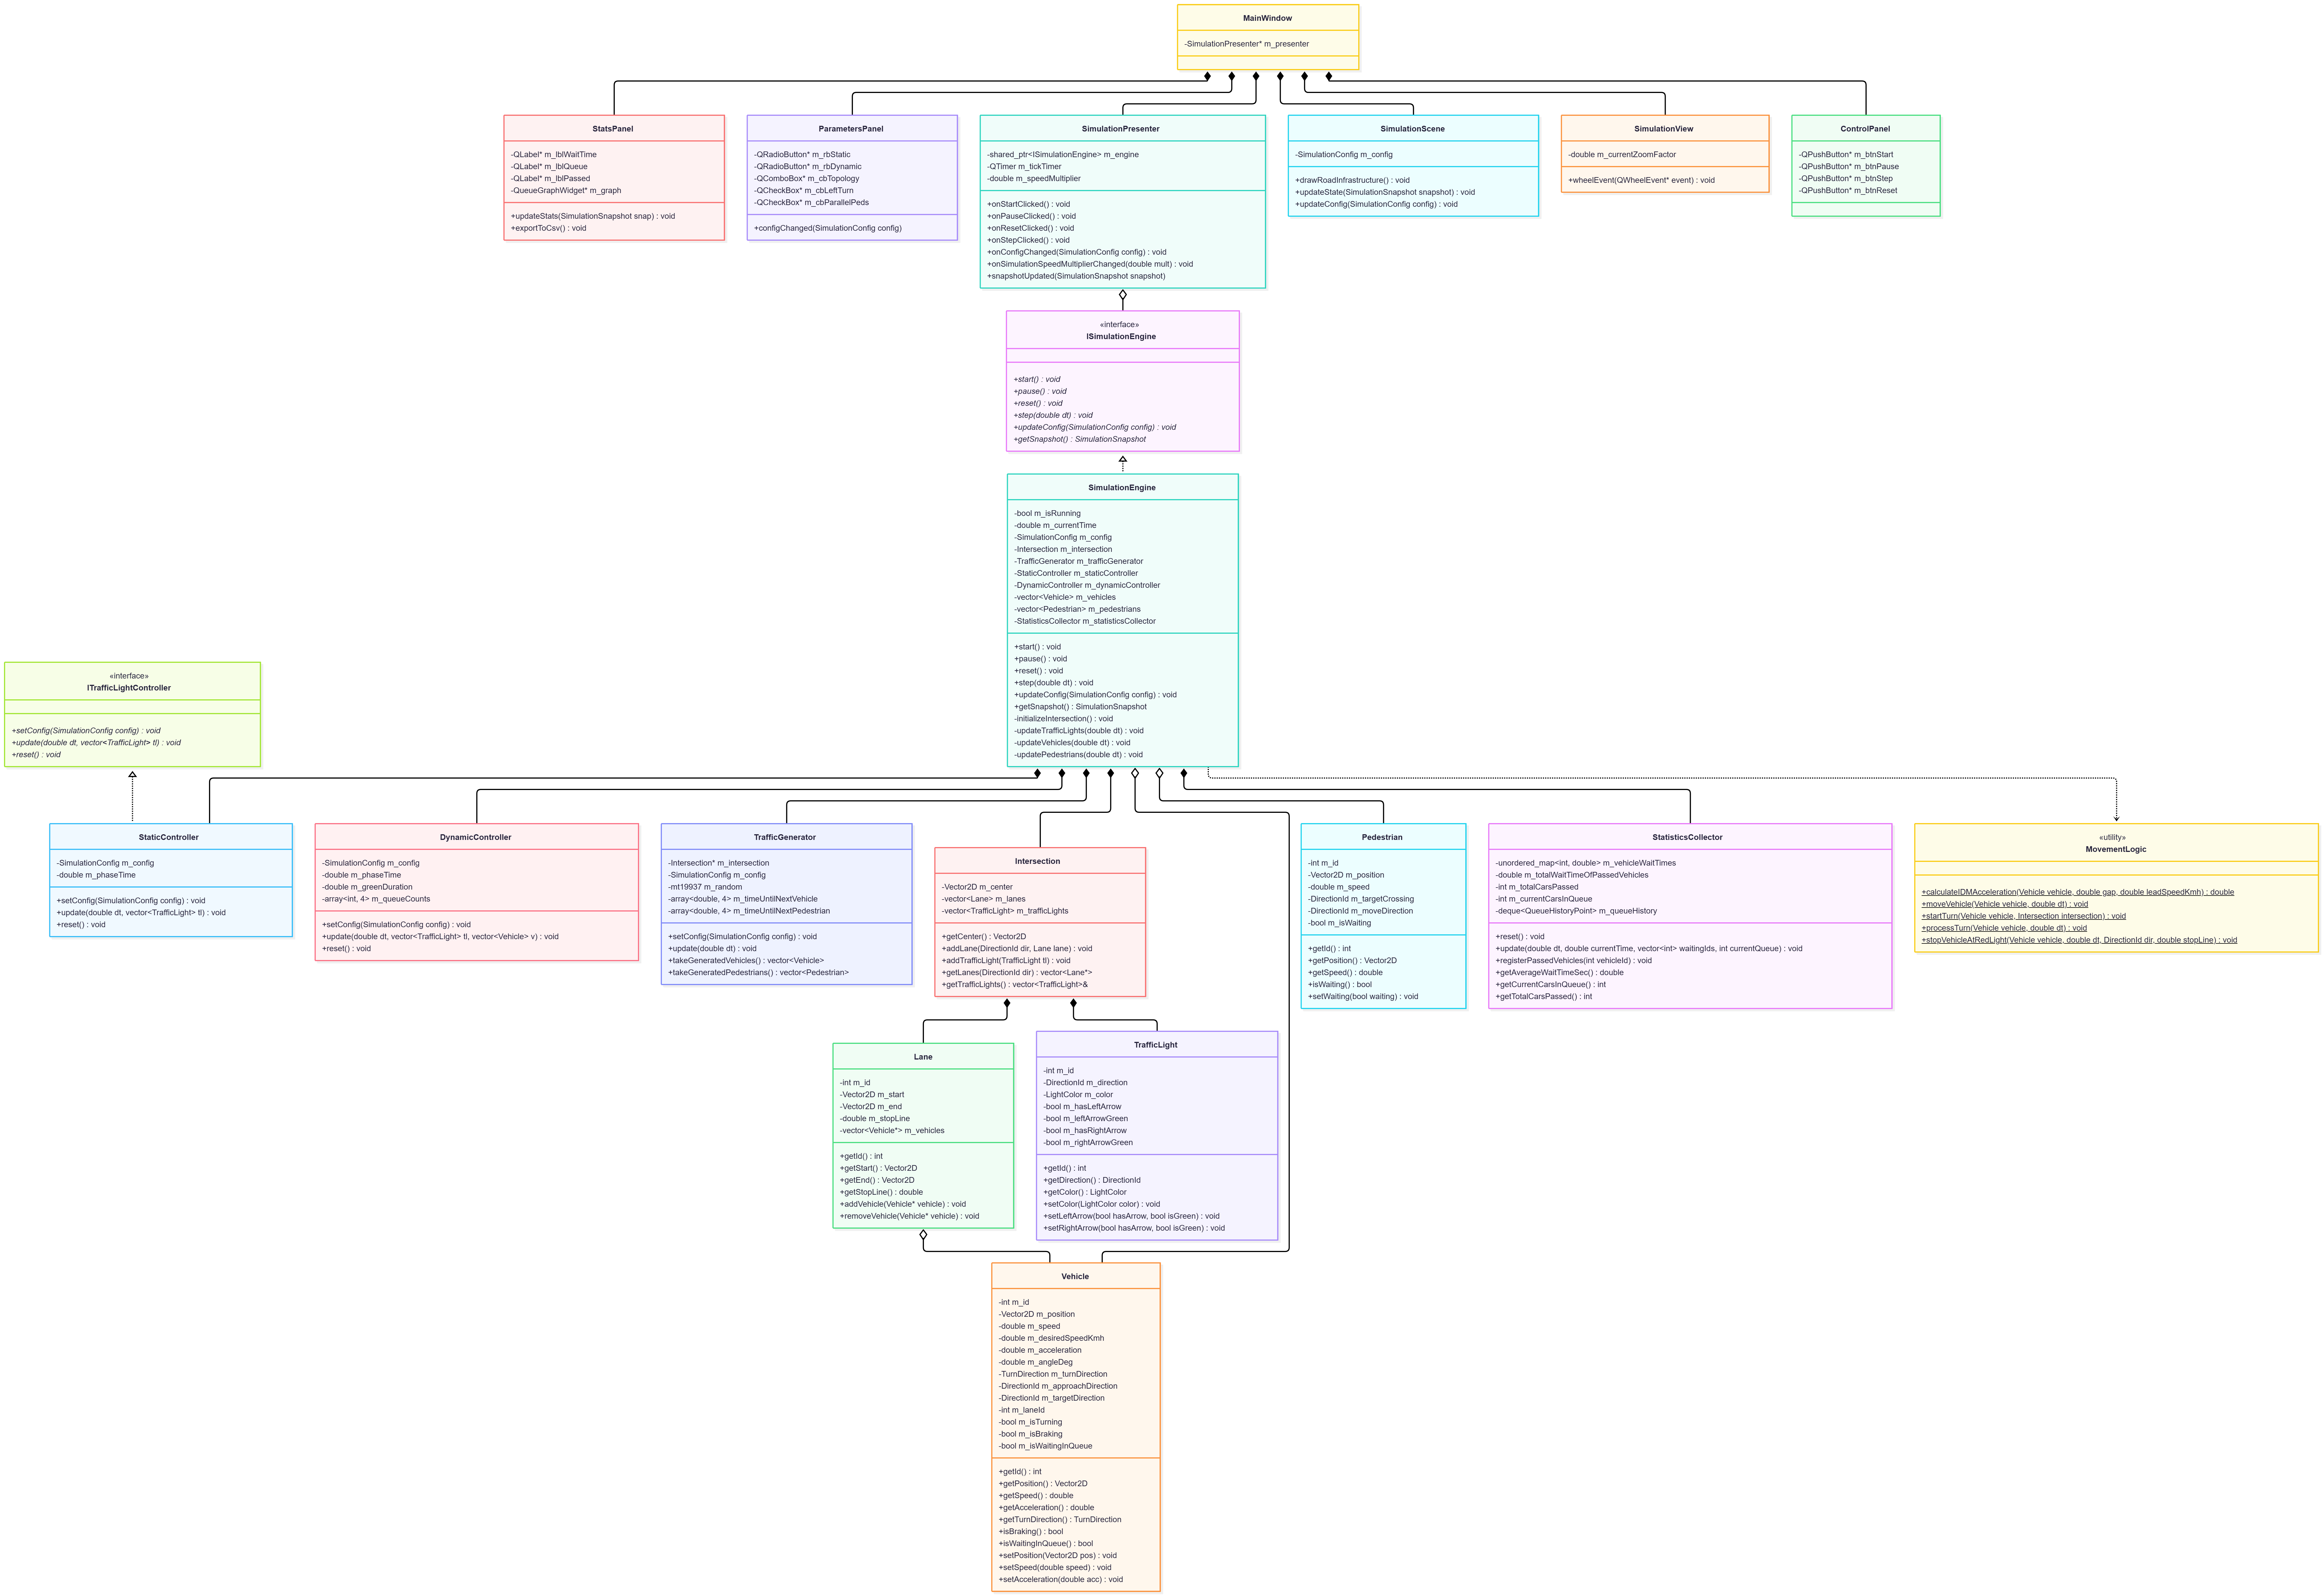
\includegraphics[width=\textwidth]{dia}
  \caption{Диаграмма классов программного комплекса моделирования перекрестка}
  \label{fig:class_diagram}
\end{figure}

\subsection{Взаимосвязи между компонентами архитектуры}
\begin{itemize}
  \item Фасадный интерфейс \texttt{ISimulationEngine} определяет методы управления симуляцией (\texttt{start}, \texttt{pause}, \texttt{step}, \texttt{reset}) и получения среза данных (\texttt{getSnapshot}).
  \item Класс \texttt{SimulationEngine} реализует интерфейс модели и объединяет модули инфраструктуры (\texttt{Intersection}), генерации (\texttt{TrafficGenerator}), управления светофорами (\texttt{StaticController}, \texttt{DynamicController}), физики движения (\texttt{MovementLogic}) и статистики (\texttt{StatisticsCollector}).
  \item Презентер \texttt{SimulationPresenter} принимает сигналы таймера с частотой 30 кадров/с, выполняет квант времени $\Delta t$ в ядре и передает снимок \texttt{SimulationSnapshot} в представление (\texttt{SimulationView}, \texttt{SimulationScene}, \texttt{StatsPanel}).
\end{itemize}

\newpage
\section{Текстовые спецификации основных классов системы}
\subsection{Модуль моделируемых сущностей (\texttt{src/core/entities/})}
\begin{itemize}
  \item \textbf{\texttt{Vehicle}}:
  \begin{itemize}
    \item \textit{Поля}: \texttt{m\_id} (уникальный номер ТС), \texttt{m\_position} (вектор координат $\vec{r}$), \texttt{m\_speed} (текущая скорость), \texttt{m\_desiredSpeedKmh} (желаемая скорость), \texttt{m\_acceleration} (ускорение $a$), \texttt{m\_angleDeg} (угол курса), \texttt{m\_turnDirection} (маневр: прямо, влево, вправо), \texttt{m\_approachDirection} (подход прибытия), \texttt{m\_targetDirection} (целевое направление), \texttt{m\_laneId} (номер полосы), \texttt{m\_isTurning} (флаг выполнения поворота), \texttt{m\_turnProgress} (прогресс прохождения дуги $[0, 1]$), \texttt{m\_turnCenter}, \texttt{m\_turnRadius}, \texttt{m\_isBraking} (флаг торможения), \texttt{m\_isWaitingInQueue} (флаг ожидания в заторе).
    \item \textit{Методы}: геттеры и сеттеры кинематического состояния, расчет углов траектории, управление флагами очередей и торможения.
  \end{itemize}
  \item \textbf{\texttt{Pedestrian}}:
  \begin{itemize}
    \item \textit{Поля}: \texttt{m\_id}, \texttt{m\_position}, \texttt{m\_speed} ($1.0$--$1.5\text{ м/с}$), \texttt{m\_targetCrossing} (целевой переход), \texttt{m\_moveDirection} (направление движения), \texttt{m\_isWaiting} (флаг ожидания разрешающего сигнала на границе тротуара).
    \item \textit{Методы}: чтение и модификация координат, скорости, направления и статуса ожидания.
  \end{itemize}
  \item \textbf{\texttt{Lane}}:
  \begin{itemize}
    \item \textit{Поля}: \texttt{m\_id}, \texttt{m\_start}, \texttt{m\_end} (геометрические координаты оси полосы), \texttt{m\_stopLine} (координата стоп-линии), \texttt{m\_vehicles} (список указателей на ТС, находящиеся на полосе).
    \item \textit{Методы}: \texttt{addVehicle(Vehicle*)}, \texttt{removeVehicle(Vehicle*)}, \texttt{getVehicles()}, \texttt{getStopLine()}.
  \end{itemize}
  \item \textbf{\texttt{TrafficLight}}:
  \begin{itemize}
    \item \textit{Поля}: \texttt{m\_id}, \texttt{m\_direction}, \texttt{m\_color} (сигналы Red, Yellow, Green, RedYellow), \texttt{m\_hasLeftArrow}, \texttt{m\_leftArrowGreen}, \texttt{m\_hasRightArrow}, \texttt{m\_rightArrowGreen}.
    \item \textit{Методы}: установка и считывание основных сигналов и дополнительных стрелочных секций.
  \end{itemize}
\end{itemize}

\subsection{Модуль физики и моделирования (\texttt{src/core/simulation/})}
\begin{itemize}
  \item \textbf{\texttt{Intersection}}:
  \begin{itemize}
    \item \textit{Поля}: \texttt{m\_center}, \texttt{m\_lanes} (вектор полос движения), \texttt{m\_lanesByDirection} (индексация полос по сторонам света), \texttt{m\_trafficLights} (вектор светофоров).
    \item \textit{Методы}: инициализация геометрии перекрестка в зависимости от выбранной топологии, выборка полос по направлению движения.
  \end{itemize}
  \item \textbf{\texttt{MovementLogic}}:
  \begin{itemize}
    \item \textit{Методы (статические)}:
    \begin{itemize}
      \item \texttt{calculateIDMAcceleration(\dots)}: расчет продольного ускорения по формуле модели IDM с учетом дистанции и скорости лидера.
      \item \texttt{moveVehicle(Vehicle\&, double dt)}: численное интегрирование скорости и координат прямолинейного движения.
      \item \texttt{startTurn(\dots)}, \texttt{processTurn(\dots)}: расчет криволинейной кинематики движения по дуге окружности.
      \item \texttt{stopVehicleAtRedLight(\dots)}: остановка автомобиля перед стоп-линией на запрещающий сигнал.
    \end{itemize}
  \end{itemize}
  \item \textbf{\texttt{TrafficGenerator}}:
  \begin{itemize}
    \item \textit{Поля}: указатель на \texttt{Intersection}, генератор псевдослучайных чисел \texttt{std::mt19937}, массив таймеров появления ТС и пешеходов \texttt{m\_timeUntilNextVehicle}, \texttt{m\_timeUntilNextPedestrian}.
    \item \textit{Методы}: \texttt{update(dt)}, генерация интервалов по экспоненциальному закону, генерация скоростей, выбор полосы спавна согласно правилам ПДД.
  \end{itemize}
  \item \textbf{\texttt{SimulationEngine}}:
  \begin{itemize}
    \item \textit{Поля}: флаг \texttt{m\_isRunning}, физическое время \texttt{m\_currentTime}, конфигурация \texttt{SimulationConfig}, экземпляры модулей ядра и контейнеры сущностей \texttt{m\_vehicles}, \texttt{m\_pedestrians}.
    \item \textit{Методы}: реализация интерфейса \texttt{ISimulationEngine}, диспетчеризация движения на шаге \texttt{step(dt)}, разрешение конфликтов встречного разъезда при левом повороте, удаление ТС, покинувших область симуляции ($> 110\text{ м}$).
  \end{itemize}
\end{itemize}

\subsection{Модуль управления светофорными объектами (\texttt{src/core/traffic\_control/})}
\begin{itemize}
  \item \textbf{\texttt{ITrafficLightController}}: интерфейс с виртуальными методами \texttt{setConfig}, \texttt{update} и \texttt{reset}.
  \item \textbf{\texttt{StaticController}}: реализует жесткую циклограмму переключения фаз с учетом промежуточных тактов (желтый $3\text{ с}$, красно-желтый $1.5\text{ с}$, пешеходная фаза).
  \item \textbf{\texttt{DynamicController}}: осуществляет опрос виртуальных детекторов очередей и производит адаптивное продление зеленой фазы шагами по $2\text{ с}$ или досрочную смену такта при рассасывании затора.
\end{itemize}

\subsection{Модуль аналитики (\texttt{src/core/analytics/})}
\begin{itemize}
  \item \textbf{\texttt{StatisticsCollector}}: ведет учет индивидуального времени задержки каждого ТС (\texttt{m\_vehicleWaitTimes}), подсчитывает суммарное число выехавших автомобилей и сохраняет кольцевой буфер истории очередей за последние 60 секунд.
\end{itemize}

\subsection{Модуль графического интерфейса (\texttt{src/ui/})}
\begin{itemize}
  \item \textbf{\texttt{SimulationPresenter}}: управляющий класс, связывающий ядро модели и графические компоненты по таймеру 30 FPS.
  \item \textbf{\texttt{SimulationView} / \texttt{SimulationScene}}: холст на базе Qt Graphics Framework с поддержкой масштабирования колесиком мыши, панорамирования и отрисовки дорожной разметки, стоп-линий, зебр, светофоров и автомобилей.
  \item \textbf{\texttt{ParametersPanel}}: док-панель параметров перекрестка с дебаунс-таймером обновления настроек.
  \item \textbf{\texttt{StatsPanel}}: док-панель вывода задержек, очередей, построения динамического графика и экспорта данных в CSV.
\end{itemize}

\section{Использованные инструментальные средства}
\begin{enumerate}
  \item \textbf{Язык программирования}: C++ (стандарт C++17). Использованы возможности стандартной библиотеки STL: алгоритмы генерации псевдослучайных величин (\texttt{<random>}), контейнеры (\texttt{std::vector}, \texttt{std::deque}, \texttt{std::unordered\_map}), умные указатели.
  \item \textbf{Графический фреймворк}: Qt 6 (модули \texttt{Qt6::Core}, \texttt{Qt6::Gui}, \texttt{Qt6::Widgets}). Применены механизмы метаобъектной системы, сигналов и слотов, графическая сцена \texttt{QGraphicsView}/\texttt{QGraphicsScene} и стилизация QSS.
  \item \textbf{Интегрированная среда разработки (IDE)}: Qt Creator.
  \item \textbf{Система автоматизации сборки}: CMake (версия $\ge 3.16$) с генератором сборочных сценариев Ninja.
  \item \textbf{Среда воспроизводимости зависимостей}: Nix / Nix-shell (\texttt{shell.nix}), обеспечивающая автоматическую изоляцию компилятора GCC, библиотек Qt6 и сборочных утилит.
  \item \textbf{Система контроля версий}: Git, удаленный хостинг исходного кода GitHub.
\end{enumerate}

\section{Описание файловой структуры программной системы}
{\footnotesize
\begin{verbatim}
TrafficSimulation/
|-- CMakeLists.txt                  # Корневой сборочный сценарий CMake
|-- shell.nix                       # Окружение зависимостей для Nix-shell
|-- .gitignore                      # Правила исключения временных файлов
|-- backend_tz.md                   # ТЗ на математическое ядро модели
|-- resources/                      # Ресурсы приложения
|   |-- resources.qrc               # XML-дескриптор ресурсов Qt
|   |-- icons/                      # SVG-иконки интерфейса (play, pause, step)
|   -- styles/
|       -- style.qss               # Таблица стилей интерфейса (QSS)
|-- src/                            # Исходный код приложения
|   |-- main.cpp                    # Точка входа в программу
|   |-- common/                     # Общие типы данных и контракты
|   |   |-- Types.h                 # Перечисления: фазы, цвета, направления
|   |   |-- Vector2D.h              # Математический 2D-вектор
|   |   |-- SimulationConfig.h      # Структура параметров моделирования
|   |   |-- ISimulationEngine.h     # Интерфейс движка и снимок Snapshot
|   |   -- MockSimulationEngine.h  # Заглушка для тестирования UI
|   |-- core/                       # Ядро модели (библиотека TrafficCore)
|   |   |-- entities/               # Моделируемые сущности
|   |   |   |-- Vehicle.h / .cpp    # Класс транспортного средства
|   |   |   |-- Pedestrian.h / .cpp # Класс пешехода
|   |   |   |-- TrafficLight.h/.cpp # Класс светофорного объекта
|   |   |   -- Lane.h / .cpp       # Класс полосы движения со стоп-линией
|   |   |-- simulation/             # Логика моделирования
|   |   |   |-- Intersection.h/.cpp # Топология перекрестка
|   |   |   |-- TrafficGenerator.h/c# Стохастический генератор потоков
|   |   |   |-- MovementLogic.h/.cpp# Физика IDM, маневры поворотов
|   |   |   -- SimulationEngine.h/c# Цикл квантования времени (dt)
|   |   |-- traffic_control/        # Алгоритмы управления светофорами
|   |   |   |-- ITrafficLightController.h # Интерфейс контроллера
|   |   |   |-- StaticController.h/c# Контроллер жестких фаз
|   |   |   -- DynamicController.h/# Адаптивный контроллер очередей
|   |   -- analytics/              # Аналитический учет
|   |       -- StatisticsCollector.h/.cpp # Подсчет задержек и очередей
|   -- ui/                         # Пользовательский интерфейс (Qt Widgets)
|       |-- mainwindow.h / .cpp/.ui # Главное окно приложения
|       |-- canvas/                 # Модуль графической сцены
|       |   |-- SimulationView.h/.cp# Представление QGraphicsView
|       |   |-- SimulationScene.h/cp# Сцена с отрисовкой перекрестка
|       |   -- items/              # Графические элементы сцены
|       |-- panels/                 # Док-панели интерфейса
|       |   |-- ControlPanel.h/.cpp # Управление (пуск, пауза, шаг)
|       |   |-- ParametersPanel.h/cp# Панель параметров симуляции
|       |   -- StatsPanel.h / .cpp # Метрики, график очереди и CSV
|       -- presenter/              # Слой связи MVP
|           -- SimulationPresenter.h/.cpp # Связывание ядра и интерфейса
-- tests/                          # Модульные тесты ядра
|-- CMakeLists.txt              # Сборка тестов
|-- test_traffic_generator.cpp  # Тестирование генератора трафика
`-- test_traffic_phases.cpp     # Тестирование бесконфликтности фаз
\end{verbatim}
}

\section{Краткая характеристика пользовательского интерфейса}
Графический интерфейс системы разработан на базе фреймворка Qt~6 Widgets в соответствии с архитектурным шаблоном Model-View-Presenter (MVP). Оформление выполнено в современной высококонтрастной темной теме посредством таблиц стилей Qt Style Sheets (\texttt{style.qss}) с акцентной синей палитрой (\texttt{\#3D5AFE}).
Компоновка главного окна включает три ключевые зоны: центральную интерактивную графическую область моделирования и две функциональные док-панели (\texttt{QDockWidget}), поддерживающие перемещение и открепление.

\subsection{Центральная графическая область (\texttt{SimulationView} / \texttt{SimulationScene})}
Графическая подсистема реализована на базе специализированного представления \texttt{Simulation\-View} (наследник \texttt{QGraphicsView}) и сцены \texttt{SimulationScene} ($200 \times 200\text{ м}$ в метрической системе координат):
\begin{itemize}
  \item \textbf{Интерактивная навигация}: реализовано плавное масштабирование сцены колесиком мыши (с коэффициентом от $0.5\times$ до $3.0\times$ с центрированием под курсором) и свободное двумерное панорамирование перетаскиванием (режим \texttt{ScrollHandDrag}).
  \item \textbf{Отрисовка дорожной инфраструктуры}:
  \begin{itemize}
    \item Проезжая часть темно-серого асфальтового оттенка (\texttt{\#2B2D42}) с двойной сплошной осевой линией желтого цвета (\texttt{\#F4D03F}), белыми прерывистыми разделителями полос и сплошными стоп-линиями толщиной $0.15\text{ м}$.
    \item Пешеходные тротуары со скругленными границами радиусом $R = 3.5\text{ м}$ на углах перекрестка.
    \item Четыре пешеходных перехода («зебры») шириной $3.0\text{ м}$ с процедурной генерацией контрастных белых полос с шагом $1.0\text{ м}$.
  \end{itemize}
  \item \textbf{Визуализация светофорных объектов}:
  \begin{itemize}
    \item \textit{Автомобильные светофоры} (\texttt{TrafficLightGraphicsItem}): трехсекционные вертикальные стойки с корпусом графитового цвета, поддерживающие динамическую индикацию основных сигналов (Red, Yellow, Green, RedYellow) и дополнительной секции стрелки левого поворота.
    \item \textit{Пешеходные светофоры} (\texttt{PedestrianTrafficLightGraphicsItem}): комплексные Г-образные опоры на всех четырех углах перекрестка, каждая из которых несет по два независимых двухсекционных излучателя для раздельной индикации переходов по направлениям «Север--Юг» и «Восток--Запад».
  \end{itemize}
  \item \textbf{Модели транспортных средств (\texttt{VehicleGraphicsItem})}:
  \begin{itemize}
    \item Масштабная геометрия кузова $4.5 \times 1.8\text{ м}$ со скруглением углов, зеркалами заднего вида, лобовым и задним остеклением со световыми бликами.
    \item Цветовое кодирование маневров: синий кузов (\texttt{\#2196F3})~--- движение прямо, оранжевый (\texttt{\#FF9800})~--- поворот налево, фиолетовый (\texttt{\#9C27B0})~--- поворот направо.
    \item Световая сигнализация: передние фары, габаритные огни, динамические стоп-сигналы ярко-красного цвета (\texttt{\#FF1744}), активирующиеся при торможении ($a < -0.5\text{ м/с}^2$), и мигающие желтые указатели поворота (период $0.66\text{ с}$, скважность $50\%$).
  \end{itemize}
  \item \textbf{Модели пешеходов (\texttt{PedestrianGraphicsItem})}: векторные диски радиусом $0.6\text{ м}$ с белой окантовкой. Двухцветная статусная индикация: ярко-зеленый цвет (\texttt{\#00E676}) сигнализирует о движении по переходу, а янтарно-желтый (\texttt{\#FFA000})~--- об ожидании разрешающего сигнала на тротуаре.
\end{itemize}

\subsection{Левая док-панель («Управление и Аналитика»)}
Панель объединяет управление воспроизведением, глобальные параметры и блок вывода аналитических метрик:
\begin{enumerate}
  \item \textbf{Блок управления симуляцией (\texttt{ControlPanel})}:
  \begin{itemize}
    \item Сегментированная панель кнопок быстрого доступа со стилизованными SVG-иконками: «Старт» (\texttt{play.svg}), «Пауза» (\texttt{pause.svg}), покадровый «Шаг» (\texttt{step\_\allowbreak forward.svg}) и «Сброс» (\texttt{stop.svg}).
    \item Цифровой регулятор скорости моделирования (\texttt{QDoubleSpinBox}) в диапазоне от $0.1\times$ до $5.0\times$ (с шагом $0.1\times$, значение по умолчанию $1.00\times$).
  \end{itemize}
  \item \textbf{Группа «Глобальные параметры»}:
  \begin{itemize}
    \item Дублированное управление через спаренные ползунки (\texttt{QSlider}) и поля ввода (\texttt{QSpinBox}):
    \begin{itemize}
      \item «Общий цикл (с)»: суммарный цикл светофорного регулирования $T \in [30, 180]\text{ с}$ (по умолчанию $90\text{ с}$).
      \item «Видимость (м)»: дальность обнаружения светофора и заторов $D \in [20, 150]\text{ м}$ (по умолчанию $60\text{ м}$).
      \item «З-ый пеш-в (с)»: длительность зеленого пешеходного сигнала $Z_{\text{ped}} \in [5, 60]\text{ с}$ (по умолчанию $15\text{ с}$).
      \item «Поток пеш-в»: общая интенсивность пешеходов $P_{\text{ped}} \in [50, 1000]\text{ пеш/ч}$ (по умолчанию $300$).
      \item «Ск-ть min (км/ч)» и «Ск-ть max (км/ч)»: допустимый диапазон скоростей ТС от $20$ до $140\text{ км/ч}$ со встроенной перекрестной валидацией ($V_{\min} \le V_{\max}$).
    \end{itemize}
    \item Автоматическая деактивация недоступных настроек (например, общего цикла $T$ и времени пешеходного зеленого $Z_{\text{ped}}$ при переключении в адаптивный режим или при совмещенной пешеходной фазе).
  \end{itemize}
  \item \textbf{Блок оперативной аналитики (\texttt{StatsPanel})}:
  \begin{itemize}
    \item Цифровые табло реального времени: «Средняя задержка» (с точностью до $0.1\text{ с}$), «Очередь (авто)» (число остановившихся ТС, $v < 0.5\text{ м/с}$) и «Проехало машин» (суммарный счетчик выбывших ТС).
    \item Встроенный графический осциллограф очередей (\texttt{QueueGraphWidget}): отображает непрерывный временной ряд длины очереди за последние $60\text{ секунд}$ со вспомогательной сеткой, динамическим масштабированием шкалы ординат (\texttt{Max Y}) и синей градиентной заливкой под кривой.
    \item Кнопка «Экспорт в CSV»: выгружает накопленный массив симуляции (\texttt{SimTimeSec}, \texttt{CarsInQueue}, \texttt{AverageWaitTimeSec}, \texttt{TotalCarsPassed}) в файл с меткой времени в директорию документов пользователя с выводом модального уведомления об успешном сохранении.
  \end{itemize}
\end{enumerate}

\subsection{Правая док-панель («Параметры»)}
Предназначена для детального конфигурирования топологии, правил разъезда и пофазных таймингов подходов:
\begin{enumerate}
  \item \textbf{Группа «Настройки перекрестка»}:
  \begin{itemize}
    \item Переключатель режима светофорного контроллера: радиокнопки «Статический» / «Адаптивный».
    \item Выпадающий список выбора топологии дорог: «2+2», «2+3 (Асимметрия)», «3+3».
    \item Чекбокс «Просачивание налево»: разрешает выполнение левого поворота во встречный разъезд.
    \item Чекбокс «Пешеходы в фазе с авто»: включает пропуск пешеходов параллельно попутному автотранспорту; блокируется при активном режиме просачивания налево для предотвращения конфликтных ситуаций.
  \end{itemize}
  \item \textbf{Группа «Светофоры (Тайминги)»}:
  \begin{itemize}
    \item Четыре специализированных блока подходов: «$\uparrow$ Север», «$\downarrow$ Юг», «$\rightarrow$ Восток», «$\leftarrow$ Запад».
    \item Для каждого направления предусмотрены независимые регуляторы (слайдер + спинбокс): интенсивность потока $P$ ($100$--$2000\text{ авт/ч}$), длительность зеленого сигнала $Z$ ($5$--$180\text{ с}$) и красного сигнала $K$ ($5$--$180\text{ с}$).
    \item \textit{Попарная синхронизация подходов}: регуляторы встречных направлений программно связаны (Север $\leftrightarrow$ Юг, Восток $\leftrightarrow$ Запад) для синхронного переключения тактов.
    \item \textit{Автоматический баланс фаз}: при изменении длительности зеленого сигнала $Z$ время красного сигнала $K$ пересчитывается автоматически с сохранением суммарной длительности фазы цикла ($Z + K = T_{\text{phase}}$).
    \item \textit{Дебаунсинг}: отправка обновленной конфигурации в расчетное ядро осуществляется через таймер задержки ($50\text{ мс}$), предотвращая избыточные пересчеты при непрерывном перемещении ползунков.
  \end{itemize}
\end{enumerate}

\section{Краткое описание проведенных экспериментов}
\textit{(Раздел подлежит заполнению по результатам проведения серии вычислительных экспериментов)}

\vspace{0.3cm}
\noindent\textbf{Программа запланированных экспериментальных исследований:}
\begin{enumerate}
  \item \textbf{Эксперимент №1. Сравнительный анализ статического и адаптивного регулирования}: исследование величины средней задержки $T_{\text{avg\_wait}}$ и динамики очередей при симметричной средней нагрузке ($P = 600\text{ авт/ч}$ по всем подходам).
  \item \textbf{Эксперимент №2. Поведение системы в условиях асимметричной пиковой нагрузки}: анализ эффективности контроллеров при заторе по оси «Север--Юг» ($P = 1200\text{ авт/ч}$) и слабом поперечном потоке по оси «Восток--Запад» ($P = 300\text{ авт/ч}$).
  \item \textbf{Эксперимент №3. Оценка влияния режима левого поворота}: сравнительный анализ пропускной способности перекрестка при маневре «просачивания» (ВСТР) и при выделенной стрелочной фазе светофора.
  \item \textbf{Эксперимент №4. Влияние фазы пропуска пешеходов}: исследование задержек правоповоротных транспортных средств при параллельном пропуске пешеходов относительно выделенной общепешеходной фазы (All-Red).
\end{enumerate}

\section{Подготовка полного GIT-репозитория проекта на GitHub}
\begin{itemize}
  \item \textbf{Ссылка на удаленный репозиторий проекта}: \ \url{https://github.com/noobisbr0/TrafficSimulation}
  \item \textbf{Структура ветвления и интеграция}:
  \begin{itemize}
    \item Ветка \texttt{main}: базовая модульная архитектура системы, корневой сборочный файл CMake, ресурсы (иконки, QSS), каркас графического интерфейса пользователя Qt6 Widgets / QGraphicsScene и фасадная заглушка \texttt{MockSimulationEngine}.
    \item Ветка бэкенда (\texttt{backend}): полная математическая реализация библиотеки \texttt{TrafficCore} (физика IDM, стохастический генератор пуассоновских потоков, адаптивный контроллер очередей, алгоритмы дуговых маневров поворотов и модуль сбора аналитики \texttt{StatisticsCollector}).
    \item Слияние веток объединяет независимые компоненты через контракт фасадного интерфейса \texttt{ISimulationEngine} без взаимных коллизий между моделью и представлением.
  \end{itemize}
\end{itemize}

\end{document}
